\documentclass[border=5mm,tikz]{standalone}

\usetikzlibrary{calc}

\begin{document}
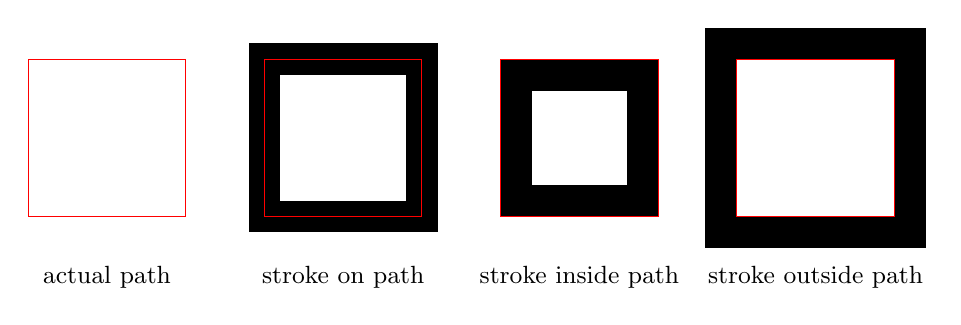
\begin{tikzpicture}[
   every node/.style = {below=5mm, text=black, font=\small},
%   scale = 1.5,
]
   % path
   \draw [red] (0,0) rectangle +(2,2)
      +(1,0) node {actual path};
   % stroke on path
   \draw [line width = 4mm] (3,0) rectangle +(2,2);
   \draw [red] (3,0) rectangle +(2,2)
      +(1,0) node {stroke on path};
   % stroke inside path
   \draw [line width = 4mm]
      ($(6,0)+(\pgflinewidth/2,\pgflinewidth/2)$) rectangle
      +($(2,2)-(\pgflinewidth,\pgflinewidth)$);
   \draw [red] (6,0) rectangle +(2,2)
      +(1,0) node {stroke inside path};
   % stroke outsie path
   \draw [line width = 4mm]
      ($(9,0)-(\pgflinewidth/2,\pgflinewidth/2)$) rectangle
      +($(2,2)+(\pgflinewidth,\pgflinewidth)$);
   \draw [red] (9,0) rectangle +(2,2)
      +(1,0) node {stroke outside path};
\end{tikzpicture}
\end{document}